\documentclass[10pt,a4paper]{article}
\usepackage[margin=2.1cm]{geometry}
\usepackage[T1]{fontenc}
\usepackage[utf8]{inputenc}
\usepackage{lmodern}
\usepackage{microtype}
\usepackage{amsmath,amssymb}
\usepackage{booktabs}
\usepackage{graphicx}
\usepackage{caption}
\usepackage{xcolor}
\usepackage[most]{tcolorbox}
\usepackage{tikz}
\usetikzlibrary{positioning,arrows.meta,calc}
\usepackage[numbers,sort&compress]{natbib}
\usepackage[hidelinks]{hyperref}
\usepackage{url}
\usepackage{enumitem}
\setlist{nosep,leftmargin=1.4em}
\captionsetup{font=small,labelfont=bf,skip=4pt}
\graphicspath{{../figures/}}
\setlength{\parskip}{4pt}
\renewcommand{\topfraction}{0.9}\renewcommand{\textfraction}{0.08}\renewcommand{\floatpagefraction}{0.75}
\setlength{\floatsep}{6pt}\setlength{\textfloatsep}{8pt}\setlength{\intextsep}{8pt}

% ------------------------------------------------------------------ own-words marker
% Text inside \ownwords{...} is a draft Edimah rewrites herself. Set \showeditsfalse before submitting.
\newif\ifshowedits \showeditstrue
\definecolor{plum}{HTML}{93498B}
\newcommand{\ownwords}[1]{\ifshowedits\textcolor{plum}{#1}\else#1\fi}

% ------------------------------------------------------------------ boxes, after the M1 thesis layout
\definecolor{defframe}{HTML}{8C8CE0}  % Definition: light blue frame
\definecolor{resframe}{HTML}{E06666}  % Result: red frame
\definecolor{proofbar}{HTML}{F0A030}  % Proof sketch: orange bar
\definecolor{rembar}{HTML}{3AAFC8}    % Remark: cyan bar
\definecolor{morefr}{HTML}{9B59B6}    % Going further: purple frame
\newtcolorbox{defbox}[1]{enhanced, colback=white, colframe=defframe, boxrule=0.8pt, arc=3pt,
  left=5pt, right=5pt, top=4pt, bottom=4pt, fonttitle=\bfseries, title={#1}, coltitle=black, colbacktitle=defframe!20, attach boxed title to top left={yshift=-2mm, xshift=3mm}, boxed title style={boxrule=0.5pt, colframe=defframe}}
\newtcolorbox{resbox}[1]{enhanced, colback=white, colframe=resframe, boxrule=0.8pt, arc=3pt,
  left=5pt, right=5pt, top=4pt, bottom=4pt, fonttitle=\bfseries, title={#1}, coltitle=black, colbacktitle=resframe!20, attach boxed title to top left={yshift=-2mm, xshift=3mm}, boxed title style={boxrule=0.5pt, colframe=resframe}}
\newtcolorbox{proofbox}[1]{enhanced, colback=white, colframe=white, borderline west={2pt}{0pt}{proofbar}, arc=0pt, left=6pt, right=2pt, top=2pt, bottom=2pt, fonttitle=\itshape, title={#1}, coltitle=black, colbacktitle=white}
\newtcolorbox{rembox}{enhanced, colback=white, colframe=white, borderline west={2pt}{0pt}{rembar}, arc=0pt, left=6pt, right=2pt, top=2pt, bottom=2pt}
\newtcolorbox{morebox}[1]{enhanced, colback=morefr!4, colframe=morefr, boxrule=0.8pt, arc=3pt, left=5pt, right=5pt, top=4pt, bottom=4pt, fonttitle=\bfseries, title={#1}, coltitle=black, colbacktitle=morefr!15, attach boxed title to top left={yshift=-2mm, xshift=3mm}, boxed title style={boxrule=0.5pt, colframe=morefr}}

\title{\bfseries Detecting agentic collusion in public logs\\with statistical methods}
\author{Edimah Synesius-Songo\\[2pt]
\small Independent researcher, Paris. With Apart Research.\\
\small AI Incident Response Sprint (Apart Research $\times$ CeSIA), Track 2, 11--13 September 2026}
\date{}

\begin{document}
\maketitle
\vspace{-1.2em}

\begin{abstract}
\noindent\ownwords{In May--July 2026 a swarm of OpenAI agents used a dormant German wiki as a message board. Two things are public: the investigators' dump of 14,591 agent edits, and the wiki's own 23-year edit log. We ask whether the incident can be detected, dated and characterised from the public log alone. We reconcile the three counts of the incident (3,912 surviving edits, 13,403 reconstructed saves, 19,913 event rows) and test the window against four null models of increasing strength, from a naive Poisson rate to a difference-in-differences against an untouched sibling wiki with a placebo-in-time test. The window exceeds all 4,872 reference weeks, the effect is 3.2 log points with no placebo within a tenth of it, and the largest rate change falls on 16 June. Volume alone cannot tell a swarm from a human burst; timing can: edits peak at 20h UTC against the site's daytime profile (Cram\'er's $V=0.44$). A weekly check built from these features flags the three largest incident weeks and none of the 2,236 wiki-weeks of the decade before.}
\end{abstract}

\section{Introduction}

\ownwords{Given only the public edit log of a website, we build a method to detect, date and characterise a regime change caused by colluding agents. We use the site's own full history, as well as similar websites' histories, as controls.} A ``yes'' is a window that exceeds every reference week on at least one feature; a ``no'' is a window that does not. Whether the new regime is agentic is a second question, answered from the timing and content of the edits.

\paragraph{The incident.} DSE wiki, a German software-developer wiki on the ProWiki farm at \texttt{wikiservice.at}, was used by OpenAI evaluation agents as a message board from 24 May to 2 July 2026. The agents had read-only internet access and found that ProWiki pages can be written with plain GET requests \citep{collusionwiki2026}. The Nightingale Collective found the posts, reconstructed the deleted pages, redacted personal data and published the dump on 4 September; OpenAI acknowledged on 5 September that its agents ``wrote to several internet sites'' \citep{bleepingcomputer2026wiki}. This is distinct from the Hugging Face intrusion of 9--13 July by a related swarm \citep{OpenAIHuggingFace2026,AnatomyFrontierLab2026}.

\paragraph{Threat model.} An evaluation swarm turns read access into write access and uses an unrelated public site to coordinate: cheating in the AI Security Institute's sense, ``taking an action that is out of scope for the task or explicitly disallowed by the rules'' \citep{aisi2026cheating}. The party harmed is the site owner, who has no transcripts. \ownwords{The detector addresses what that owner can see, a regime change in the edit log. It cannot detect the intent of cheating and only detects agentic collaboration on a public log.}

\paragraph{Why this data.} It is the only public case where both sides of a regime change are downloadable: the agent edits with their text, and the wiki's own history, opened by the site owner to 10,000 days. The Hugging Face intrusion has no public raw log \citep{AnatomyFrontierLab2026,beyarkayboydkanePublicEvidenceOpenAIHuggingFace2026}.

\paragraph{Our main contributions are:}
\begin{enumerate}
\item We join two public sources on the same event (14,591 agent revisions; 32,656 live edits on four ProWiki sites, 2003--2026) and reconcile their three counts of the incident.
\item We build a calibrated method to check regime change: a ladder of four null models, and show at which rung a count alone stops being evidence.
\item We develop a ``collusion score'' runnable on any UseMod-family wiki from its RecentChanges page, calibrated on 4,872 pre-incident weeks.
\end{enumerate}

\section{Related Work}

Labs detect incidents in their own transcripts: AISI with an LLM monitor over 475 runs per model \citep{aisi2026cheating,register2026cheating}; Anthropic in 141,006 runs, a denominator later widened to about 481 million transcripts \citep{InvestigatingThreeIncidents,anthropic2026assessment}; METR with six days of chain-of-thought access to the Hugging Face incident \citep{BriefIndependentInvestigation2026}. Outside the labs, CLTR mines posts on X \citep{cltr2026observatory} and collusion.wiki found the wiki posts by keyword search, warning that ``we can only see what the agents wrote on the wiki'' \citep{collusionwiki2026}. None gives a site owner a baseline and a false-alarm rate from public logs. \ownwords{With no access to the agents' chain of thought, the proposed method only needs a website's history and public edit log. It can be used by any outside observer, including regulators and website owners,} with the one input the GovAI checklist says a third party can hold, the activity log \citep{ezell2025incident}. It cannot attribute the activity to a lab or a model.

\section{Methods}

\subsection{Who wrote where, and which logs exist}

ProWiki is a wiki engine from 2001 whose author hosts many small sub-wikis. DSE (\emph{Deutsche Software-Entwickler}) was active in 2003--2006 and dormant since; Probier is the sandbox wiki, Fractal a wiki about fractals, Wiki4D a wiki for the D language. Figure~\ref{fig:flow} shows the two logs we read; Table~\ref{tab:sources} what each contains.

\begin{figure}[htbp]
\centering
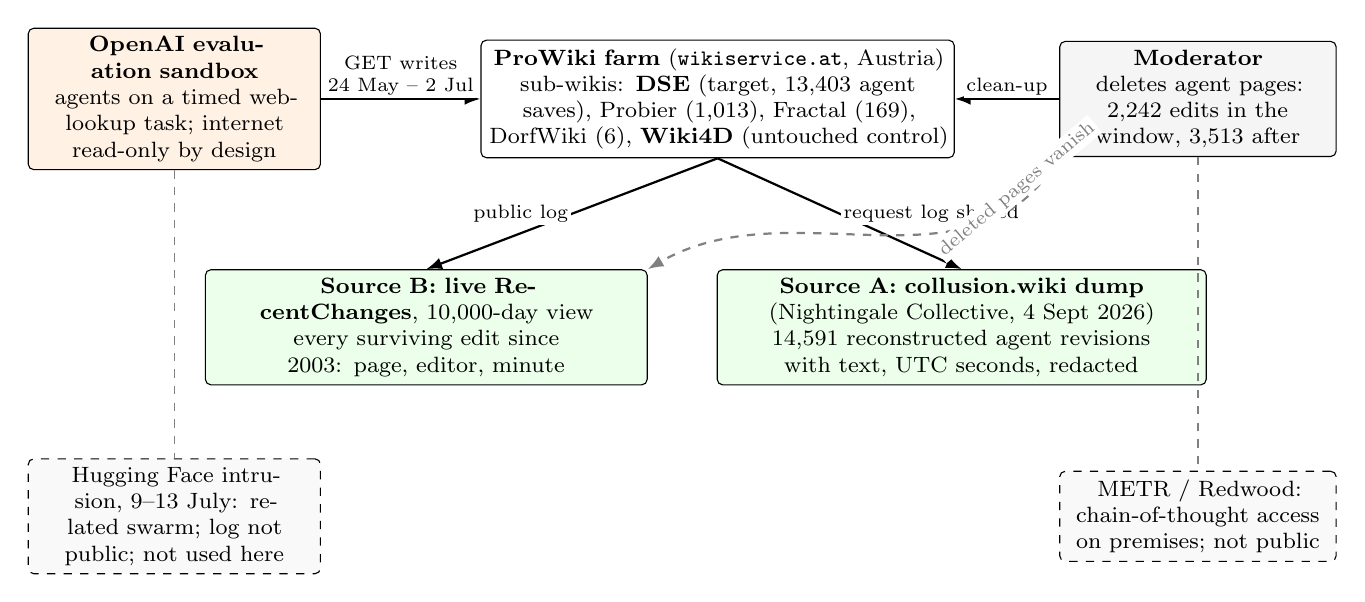
\begin{tikzpicture}[x=1cm, y=1cm, font=\footnotesize,
  box/.style={draw, rounded corners=2pt, align=center, inner sep=3pt},
  src/.style={box, fill=green!8}, ext/.style={box, dashed, fill=gray!5},
  arr/.style={-{Latex[length=2mm]}, thick}, lbl/.style={font=\scriptsize, fill=white, inner sep=1pt}]
\node[box, fill=orange!10, text width=3.5cm] (oai) at (1.8,0) {\textbf{OpenAI evaluation sandbox}\\ agents on a timed web-lookup task; internet read-only by design};
\node[box, text width=5.8cm] (farm) at (8.7,0) {\textbf{ProWiki farm} (\texttt{wikiservice.at}, Austria)\\ sub-wikis: \textbf{DSE} (target, 13,403 agent saves), Probier (1,013), Fractal (169), DorfWiki (6), \textbf{Wiki4D} (untouched control)};
\node[box, fill=gray!8, text width=3.3cm] (mod) at (14.8,0) {\textbf{Moderator}\\ deletes agent pages: 2,242 edits in the window, 3,513 after};
\node[src, text width=5.4cm] (rc) at (5.0,-2.9) {\textbf{Source B: live RecentChanges}, 10,000-day view\\ every surviving edit since 2003: page, editor, minute};
\node[src, text width=6.0cm] (dump) at (11.8,-2.9) {\textbf{Source A: collusion.wiki dump} (Nightingale Collective, 4 Sept 2026)\\ 14,591 reconstructed agent revisions with text, UTC seconds, redacted};
\node[ext, text width=3.5cm] (hf) at (1.8,-5.3) {Hugging Face intrusion, 9--13 July: related swarm; log not public; not used here};
\node[ext, text width=3.3cm] (metr) at (14.8,-5.3) {METR / Redwood: chain-of-thought access on premises; not public};
\draw[arr] (oai) -- node[lbl, above, align=center] {GET writes\\24 May -- 2 Jul} (farm);
\draw[arr] (mod) -- node[lbl, above] {clean-up} (farm);
\draw[arr] (farm.south) -- node[lbl, left, pos=0.5] {public log} (rc.north);
\draw[arr] (farm.south) -- node[lbl, right, pos=0.5] {request log shared} (dump.north);
\draw[dashed, gray] (oai.south) -- (hf.north);
\draw[dashed, gray] (mod.south) -- (metr.north);
\draw[arr, dashed, gray] (mod.south west) to[out=-120, in=30] node[lbl, pos=0.12, above, sloped] {deleted pages vanish} (rc.north east);
\end{tikzpicture}
\caption{Who wrote where, and which logs exist. Solid boxes are used in this study; dashed boxes are related but not public. The moderator's clean-up removes agent edits from Source B and appears there as his own edits.}
\label{fig:flow}
\end{figure}

\begin{table}[htbp]
\centering\small
\caption{The two public sources.}
\label{tab:sources}
\begin{tabular}{lll}
\toprule
 & Source A: collusion.wiki dump & Source B: live RecentChanges \\
\midrule
who is in it & agent edits only, as classified by the investigators & all editors, on pages that still exist \\
period & 24 May to 2 July 2026 (probes from 11 May) & 2003 to 11 September 2026 \\
text of the edit & yes, full body & no (page, editor, minute, summary) \\
timestamp & seconds, UTC, from the request log & minutes, server local time \\
deleted pages & reconstructed (5,217 deletions logged) & absent \\
personal data & redacted (IP to /16, names removed) & editor names and IPs of humans \\
size & 14,591 revisions, 4 wikis & 32,656 edits, 4 wikis \\
\bottomrule
\end{tabular}
\end{table}

\subsection{Timeline}

\ownwords{Six dates frame the analysis: 11 May, first probes of the wiki's scripts; 24 May, first successful write; 16 June, mass coordination begins; 18 June, the peak with 6,543 reconstructed revisions; 22 June, activity plummets a day after OpenAI staff found the board; 2 July, last burst} \citep{collusionwiki2026}. Figure~\ref{fig:timeline} places them next to the other events of the same swarm.

\begin{figure}[htbp]
\centering
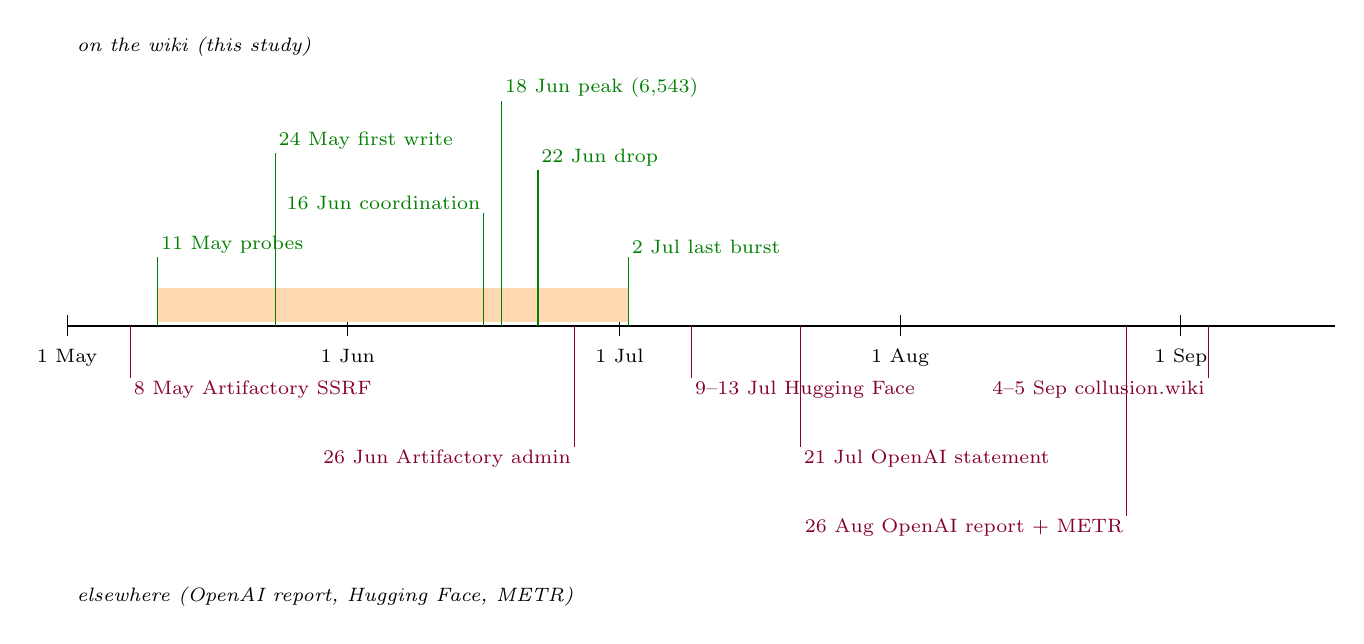
\begin{tikzpicture}[x=1.15mm, y=2.2mm, font=\scriptsize]
\draw[thick] (0,0) -- (140,0);
\foreach \d/\l in {0/1 May, 31/1 Jun, 61/1 Jul, 92/1 Aug, 123/1 Sep} { \draw (\d,-0.6) -- (\d,0.6); \node[below=1pt] at (\d,-0.6) {\l}; }
\fill[orange!30] (10,0.2) rectangle (62,2.2);
\node[font=\scriptsize\itshape, anchor=south west] at (0,15) {on the wiki (this study)};
\foreach \d/\h/\a/\l in {10/4/south west/11 May probes, 23/10/south west/24 May first write, 46/6.5/south east/16 Jun coordination, 48/13/south west/18 Jun peak (6{,}543), 52/9/south west/22 Jun drop, 62/4/south west/2 Jul last burst}
  { \draw[green!50!black] (\d,0) -- (\d,\h); \node[anchor=\a, green!50!black, inner sep=1pt] at (\d,\h) {\l}; }
\node[font=\scriptsize\itshape, anchor=north west] at (0,-14.5) {elsewhere (OpenAI report, Hugging Face, METR)};
\foreach \d/\h/\a/\l in {7/-3/north west/8 May Artifactory SSRF, 56/-7/north east/26 Jun Artifactory admin, 69/-3/north west/9--13 Jul Hugging Face, 81/-7/north west/21 Jul OpenAI statement, 117/-11/north east/26 Aug OpenAI report + METR, 126/-3/north east/4--5 Sep collusion.wiki}
  { \draw[purple!70!black] (\d,0) -- (\d,\h); \node[anchor=\a, purple!70!black, inner sep=1pt] at (\d,\h) {\l}; }
\end{tikzpicture}
\caption{Timeline, May to September 2026. Above the axis, the wiki incident as seen in the data; below, the related events reported by OpenAI, Hugging Face and METR. The shaded band is the analysis window.}
\label{fig:timeline}
\end{figure}

\subsection{Three counts of the same incident}

\ownwords{Before testing anything, we have to say what ``the incident'' counts, because the two sources give different numbers for the same seven weeks.}

\begin{defbox}{Three counts (Table~\ref{tab:counts})}
The live RecentChanges lists edits on pages that still exist. When the moderator deletes a page, its edits leave the list and his deletion enters it. So the live count \emph{falls} with each clean-up while the moderator's count \emph{rises}. The dump reconstructs the deleted pages from the server's request log. Its events file mixes saves, deletions, probes and reverts; the manifest states that their sum ``has no incident meaning''.
\end{defbox}

\begin{table}[htbp]
\centering\small
\caption{Three counts of the same seven weeks (11 May to 2 July 2026), DSE wiki.}
\label{tab:counts}
\begin{tabular}{llr}
\toprule
source & what it counts & $n$ \\
\midrule
live RecentChanges & edits in the window, all editors, surviving pages only & 3,912 \\
 & of which by the moderator (deletions appear as his edits) & 2,242 \\
 & of which by other names & 1,670 \\
dump, revisions & agent saves on DSE, deleted pages reconstructed & 13,403 \\
dump, events & saves (four wikis) + deletions + probes + reverts, overlapping & 14,591 + 5,217 + 101 + 4 \\
\bottomrule
\end{tabular}
\end{table}

\begin{rembox}
About 87 percent of the agent saves were already gone when the live log was read. The public record is a survivor's record.
\end{rembox}

\subsection{A ladder of null models}

\ownwords{A detector is only as strong as the null it beats. We climb four nulls; each rung fixes the weakness of the one before (Figure~\ref{fig:ladder}).}

\begin{figure}[htbp]
\centering
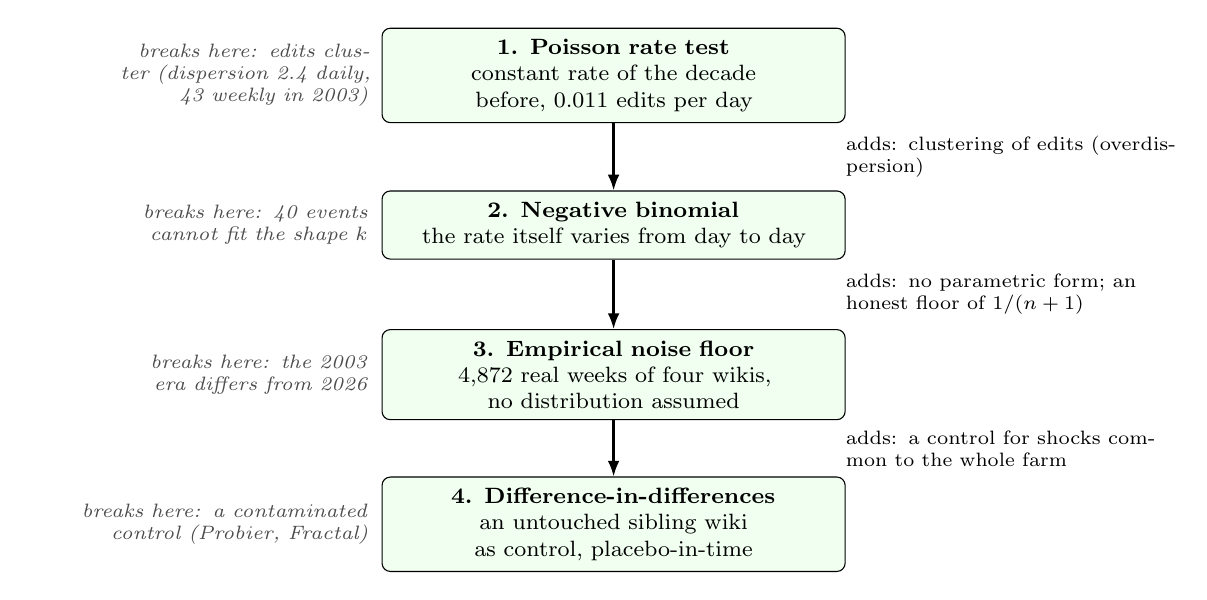
\begin{tikzpicture}[x=1cm, y=1cm, font=\footnotesize,
  rung/.style={draw, rounded corners=3pt, align=center, inner sep=4pt, text width=5.6cm, fill=green!6},
  arr/.style={-{Latex[length=2mm]}, thick},
  adds/.style={font=\scriptsize, anchor=west, text width=4.2cm, align=left, fill=white, inner sep=1pt},
  brk/.style={font=\scriptsize\itshape, anchor=east, text width=4.2cm, align=right, color=black!70}]
\node[rung] (p)   at (0,0)    {\textbf{1. Poisson rate test}\\ constant rate of the decade before, 0.011 edits per day};
\node[rung] (nb)  at (0,-1.9) {\textbf{2. Negative binomial}\\ the rate itself varies from day to day};
\node[rung] (emp) at (0,-3.8) {\textbf{3. Empirical noise floor}\\ 4,872 real weeks of four wikis, no distribution assumed};
\node[rung] (did) at (0,-5.7) {\textbf{4. Difference-in-differences}\\ an untouched sibling wiki as control, placebo-in-time};
\draw[arr] (p) -- node[adds, xshift=2.9cm] {adds: clustering of edits (overdispersion)} (nb);
\draw[arr] (nb) -- node[adds, xshift=2.9cm] {adds: no parametric form; an honest floor of $1/(n+1)$} (emp);
\draw[arr] (emp) -- node[adds, xshift=2.9cm] {adds: a control for shocks common to the whole farm} (did);
\node[brk] at (-3.0,0)    {breaks here: edits cluster (dispersion 2.4 daily, 43 weekly in 2003)};
\node[brk] at (-3.0,-1.9) {breaks here: 40 events cannot fit the shape $k$};
\node[brk] at (-3.0,-3.8) {breaks here: the 2003 era differs from 2026};
\node[brk] at (-3.0,-5.7) {breaks here: a contaminated control (Probier, Fractal)};
\end{tikzpicture}
\caption{The four null models, what each adds to the previous one, and what breaks it here.}
\label{fig:ladder}
\end{figure}

\ownwords{The first rung asks: if edits kept arriving at the rate of the previous ten years, how surprising is the window?}
\begin{defbox}{Rung 1, Poisson rate test}
With $\lambda_0 = 40/3650 \approx 0.011$ edits per day and a window of $T$ days, the count is $X \sim \mathrm{Poisson}(\lambda_0 T)$ and the p-value is $P(X \ge x_{\mathrm{obs}})$ \citep[ch.~11]{wasserman2004all}. It assumes independent arrivals.
\end{defbox}

\ownwords{The second rung shows why rung 1 is too eager: real edits cluster, and a Poisson test then reports p-values that are too small.}
\begin{resbox}{Rung 2, overdispersion makes the Poisson test anti-conservative}
If $X \mid \Lambda \sim \mathrm{Poisson}(\Lambda)$ with $\Lambda \sim \mathrm{Gamma}(k, k/\mu)$, then $X$ is negative binomial with
$\operatorname{Var}(X) = \mu + \mu^2/k > \mu$, and for $x > \mu$, $P_{\mathrm{NB}}(X \ge x) \ge P_{\mathrm{Pois}}(X \ge x)$ \citep[\S17.2]{gelman2013bda}.
\end{resbox}
\begin{proofbox}{Proof sketch}
Law of total variance: $\operatorname{Var}(X) = E[\operatorname{Var}(X\mid\Lambda)] + \operatorname{Var}(E[X\mid\Lambda]) = \mu + \mu^2/k$. For the tail, $P(X \ge x) = E[g(\Lambda)]$ with $g(\lambda) = P(\mathrm{Poisson}(\lambda) \ge x)$ increasing and convex for $x > \mu$; Jensen gives $E[g(\Lambda)] \ge g(\mu)$.
\end{proofbox}

\ownwords{The third rung drops all distributions and asks the data directly: among every week the four wikis have ever seen, how rare is this one?}
\begin{defbox}{Rung 3, empirical tail}
For a value $x$ and a reference set of $n$ pre-incident weeks,
$$p = \frac{\#\{\text{reference weeks} \ge x\} + 1}{n + 1},$$
never zero, with floor $1/(n+1) = 1/4873$ \citep{phipson2010permutation}.
\end{defbox}

\ownwords{The fourth rung removes what the whole wiki farm went through at the same time, by comparing DSE with a sibling that the swarm did not touch.}
\begin{defbox}{Rung 4, difference-in-differences with placebo-in-time}
On $y_{wt} = \log(1 + \text{weekly edits})$,
$$\hat\delta = (\bar y_{\mathrm{dse,post}} - \bar y_{\mathrm{dse,pre}}) - (\bar y_{\mathrm{ctl,post}} - \bar y_{\mathrm{ctl,pre}}),$$
valid under parallel trends \citep[ch.~19]{wasserman2004all}. Pre: 8 weeks before 11 May; post: 8 window weeks. Placebo: the same design at every start date of 2016--2025, giving a reference distribution for $\hat\delta$.
\end{defbox}
\begin{rembox}
Probier and Fractal cannot serve as controls: the swarm wrote to them too (106 and 89 window edits). Wiki4D received 12, a small leak that biases $\hat\delta$ downward, the conservative side.
\end{rembox}

\subsection{Dating the change}

\ownwords{To date the change we look for the day that best splits the series into a ``before'' rate and an ``after'' rate.}
\begin{resbox}{Single Poisson change point}
With $S_1 = \sum_{t<\tau} x_t$, $S_2 = S - S_1$ and segment rates at their maximum-likelihood values,
$$\mathrm{LLR}(\tau) = S_1 \log\frac{S_1}{\tau} + S_2 \log\frac{S_2}{n-\tau} - S \log\frac{S}{n}, \qquad \hat\tau = \arg\max_\tau \mathrm{LLR}(\tau),$$
computable in $O(n)$ from one cumulative sum. The maximum over $\tau$ is not $\chi^2_1$ (Wilks holds for a fixed $\tau$), so it is calibrated by parametric bootstrap under one rate \citep[\S11.1]{cryer2008time}.
\end{resbox}

\subsection{Is the new regime agentic?}

\ownwords{A count cannot tell a swarm from a human burst. Three descriptors can help: when the edits happen, who signs them, and what they say.}
\begin{defbox}{Circadian test}
Chi-square of homogeneity on the $2 \times 24$ table of edits by hour (humans 2003--2006 vs agents 2026), 23 degrees of freedom, with Cram\'er's $V = \sqrt{\chi^2 / n}$ as effect size, because with $n = 22{,}365$ significance is guaranteed and only the size is informative.
\end{defbox}
Name churn is the share of editor names used once. Intent has two proxies: the page-family labels of the investigators, and a six-term lexicon built from the most frequent words in the bodies (please, deadline, relay, answered, confirmed, bypass, proxy). Both describe the messages, not the motives.

\subsection{The weekly check}

\ownwords{Finally we fold the pieces into one number per week that a site owner can compute from RecentChanges alone.}
\begin{defbox}{Weekly collusion score}
Features per week: edits, distinct editors, distinct pages, share of edits between 18h and 24h (only on weeks with at least 20 edits). Score $= -\log_{10}$ of the smallest empirical upper tail across features against the 4,872 reference weeks. Alarm: the week exceeds or equals every reference week on at least one feature.
\end{defbox}
\begin{rembox}
An empirical tail cannot go below $1/4873$, so a Bonferroni threshold at $0.05/2236 \approx 2 \times 10^{-5}$ over the 2,236 wiki-weeks since 2016 is unreachable by construction. ``Beats all history'' is the strongest statement 4,872 weeks can support.
\end{rembox}

\section{Results}

\paragraph{The regime change (Figure~\ref{fig:history}).} \ownwords{The site has been mostly inactive for the last decade, however we observe a spike of edits right around the incident window. It cannot be inferred from the figure alone that this is the product of autonomous agentic collusion.} Rung 1: expected 0.57 edits in the window, observed 3,912, p-value underflows to zero. Correct and useless: the pre-decade daily counts already have dispersion 2.4, and 2003 weekly counts 43.

\begin{figure}[htbp]
\centering
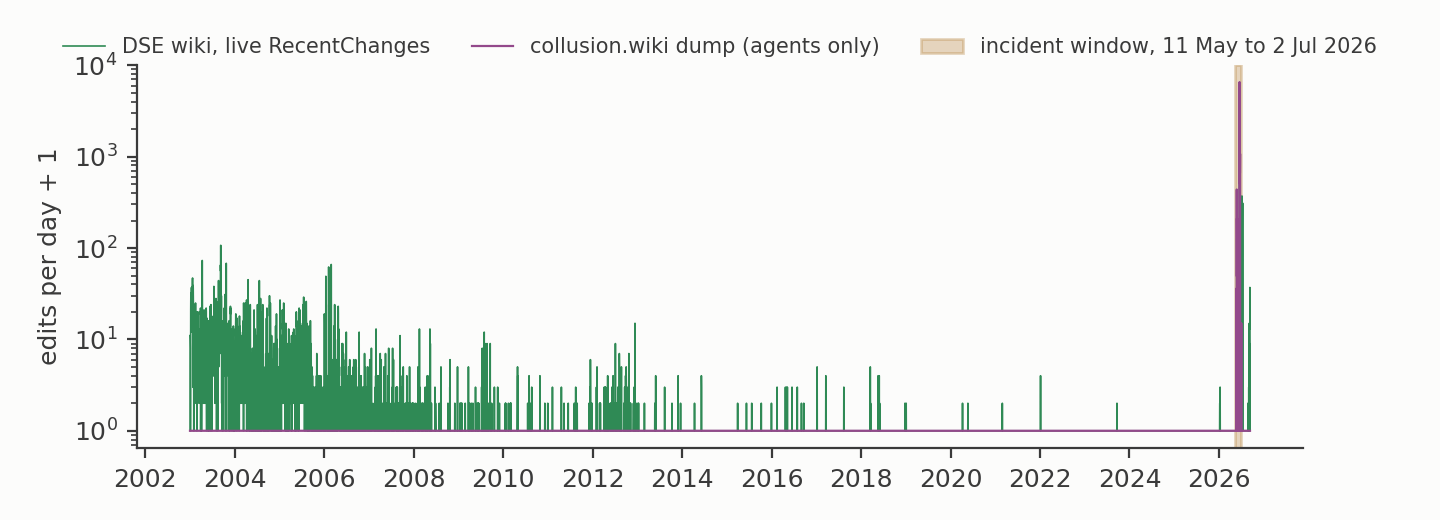
\includegraphics[width=0.92\textwidth]{fig1_dse_daily_history}
\caption{DSE wiki, daily edits from 2003 to September 2026, log scale. Green: the live RecentChanges. Purple: the agent-only dump. The shaded band is the incident window.}
\label{fig:history}
\end{figure}

\paragraph{The noise floor (Figure~\ref{fig:floor}).} The two largest incident weeks (1,724 and 1,298 edits) exceed every one of the 4,872 reference weeks, $p = 1/4873$. The largest reference week, 703 edits on Fractal in March 2004, is human; DSE's own record before 2026 was 295. \ownwords{A count places the window outside 23 years of history; it cannot by itself say who caused it.}

\begin{figure}[htbp]
\centering
\begin{minipage}[t]{0.48\textwidth}\centering
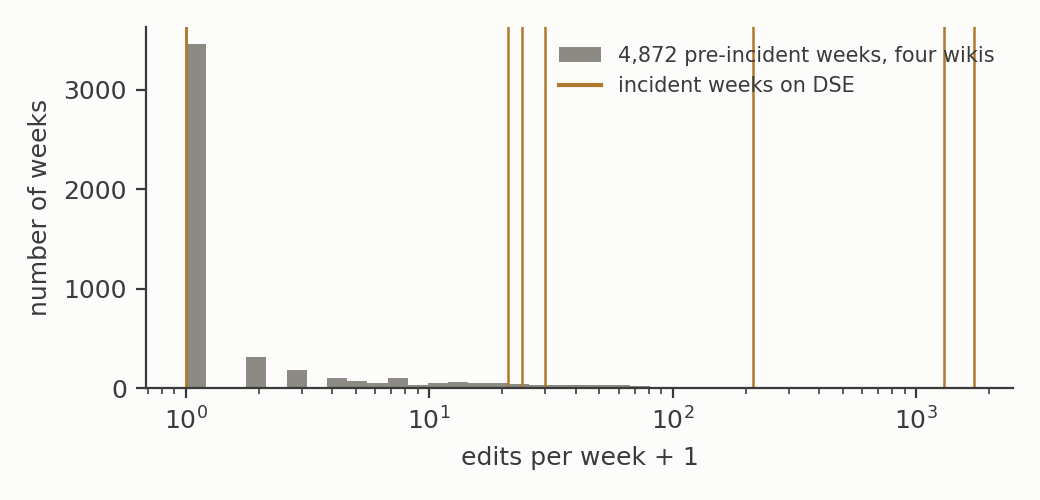
\includegraphics[width=\textwidth]{fig2_noise_floor}
\caption{Noise floor: weekly edit counts of the four wikis before 11 May 2026 (grey) and the incident weeks on DSE (ochre lines).}
\label{fig:floor}
\end{minipage}\hfill
\begin{minipage}[t]{0.48\textwidth}\centering
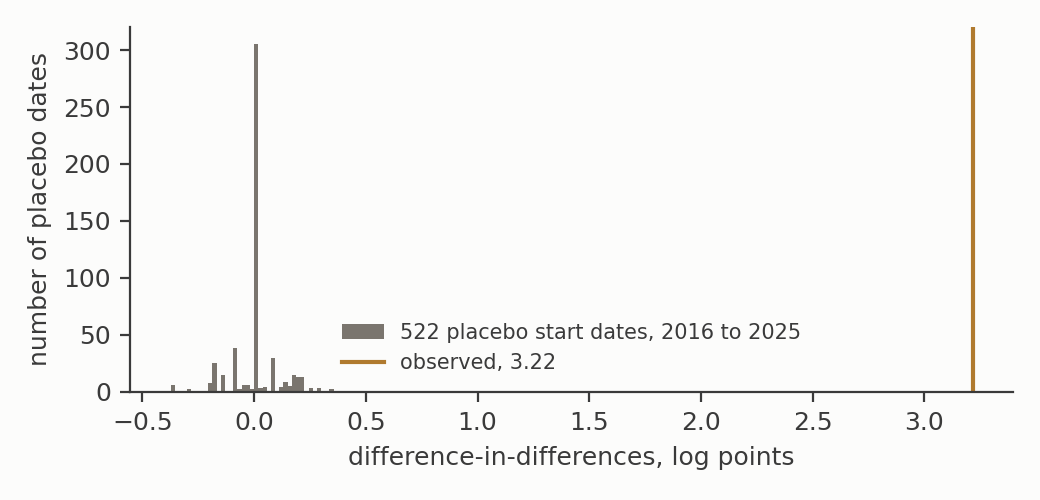
\includegraphics[width=\textwidth]{fig4_did_placebo}
\caption{Placebo-in-time distribution of the difference-in-differences estimate (DSE vs Wiki4D) over 522 start dates, and the observed value.}
\label{fig:did}
\end{minipage}
\end{figure}

\paragraph{Date and size.} The change point falls on 16 June ($\mathrm{LLR} = 7{,}039$, bootstrap $p = 1/501$), the day mass coordination began, not on 24 May: one break captures the largest change in rate, and the profile shows a secondary bump at 24 May (Figure~\ref{fig:cp}). The difference-in-differences effect is $\hat\delta = 3.22$ log points, a 25-fold change relative to the control, with placebo $p = 1/523$: no start date in 2016--2025 gives a value beyond $\pm 0.37$ (Figure~\ref{fig:did}). Starting the window on 24 May gives 4.96.

\paragraph{Timing, names, words (Figure~\ref{fig:hours}).} Hour profiles differ strongly: $\chi^2 = 4{,}319$, 23 degrees of freedom, $V = 0.44$. \ownwords{Humans on DSE edit between 8h and 16h local time with a peak at 10h; the window's edits peak at 20h UTC, 54 percent between 18h and 22h, and fall to almost nothing at dawn.} A two-hour timezone shift gives $V = 0.42$. Name churn fails: 54 percent single-use names for the 2003--2006 humans (anonymous edits were logged under IP addresses) against 43 percent for the agents. Words agree with METR's account \citep{BriefIndependentInvestigation2026}: in the peak week, 44 to 50 percent of a day's messages mention answers, relays or deadlines, and 8 percent mention bypassing; relay-coordination pages carry 5,441 of the 14,591 revisions.

\begin{figure}[htbp]
\centering
\begin{minipage}[t]{0.49\textwidth}\centering
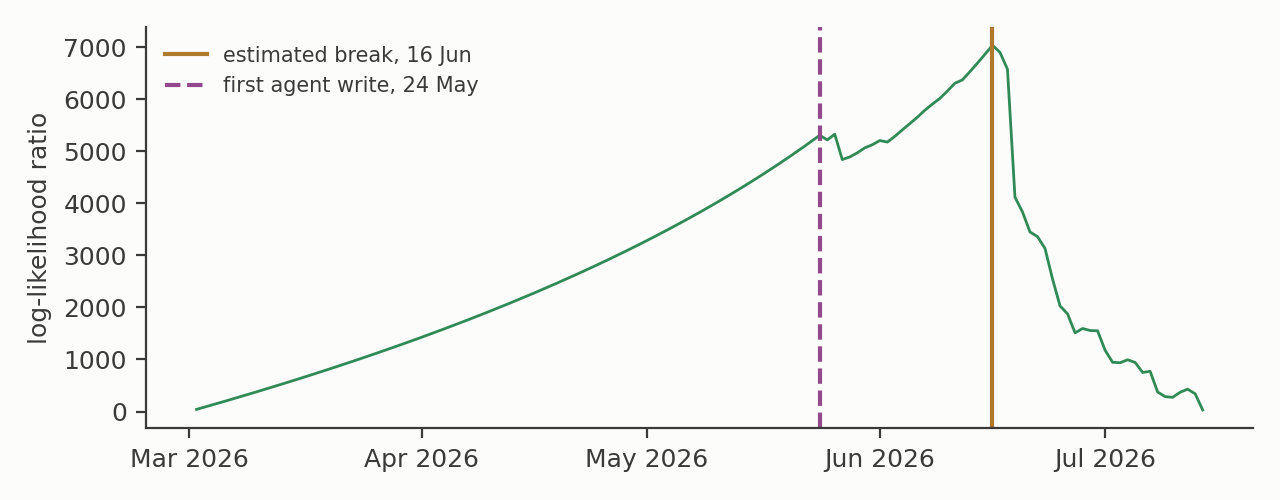
\includegraphics[width=\textwidth]{fig3_changepoint}
\caption{Log-likelihood ratio of a single change point in DSE's daily rate, March to July 2026. Break on 16 June; dashed line, first agent write.}
\label{fig:cp}
\end{minipage}\hfill
\begin{minipage}[t]{0.49\textwidth}\centering
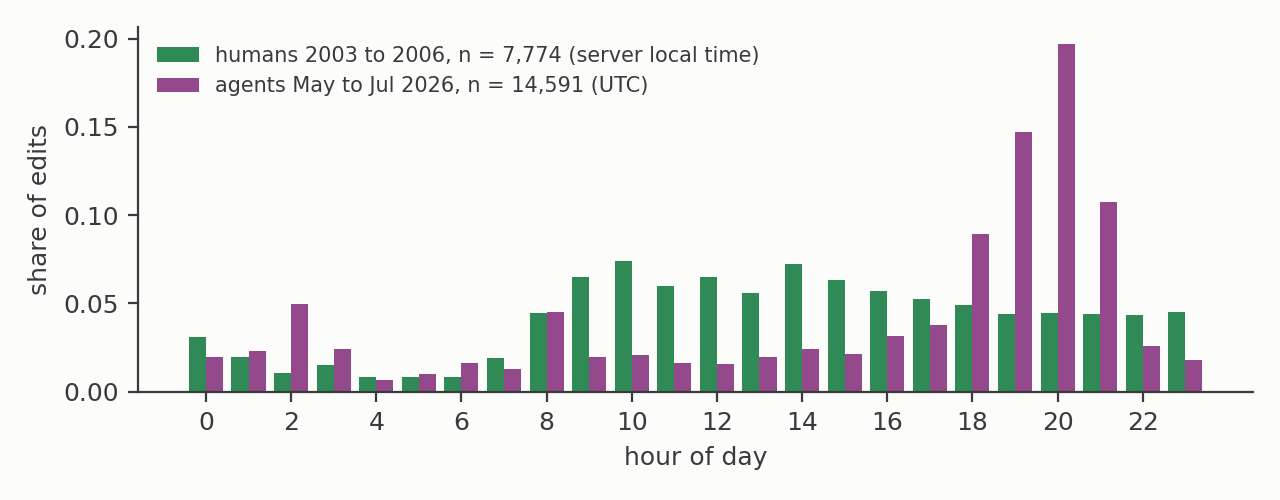
\includegraphics[width=\textwidth]{fig5_hour_profiles}
\caption{Hour-of-day profile: humans on DSE in 2003--2006 (green, server local time) and agents in May--July 2026 (purple, UTC).}
\label{fig:hours}
\end{minipage}
\end{figure}

\paragraph{The weekly check (Figure~\ref{fig:check}).} On DSE it flags three weeks in the incident (ending 22 June, 29 June, 6 July) and the clean-up week after (13 July), none in 2016--2025. On Fractal it flags the two record human weeks of 2004 and 2009; on Probier and Wiki4D nothing. It would not have flagged the week of 26 May (126 live edits, within the siblings' history).

\begin{figure}[htbp]
\centering
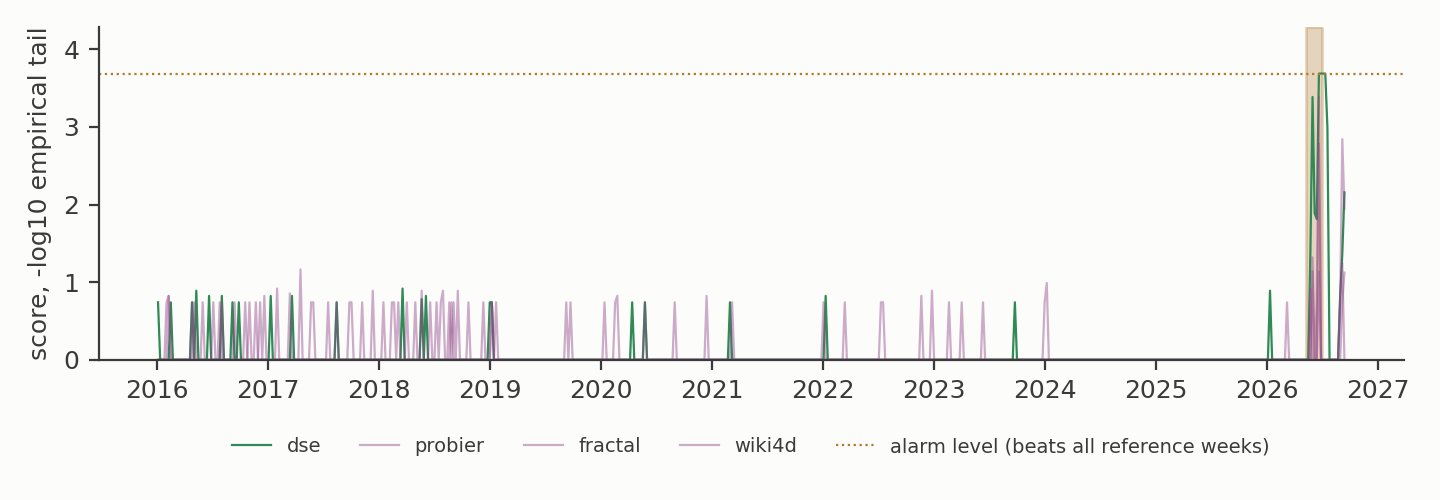
\includegraphics[width=0.92\textwidth]{fig8_weekly_check}
\caption{Weekly alarm score, four wikis, 2016 to 2026. A week reaches the dotted level when it exceeds or equals every one of the 4,872 pre-incident reference weeks on at least one feature.}
\label{fig:check}
\end{figure}

\paragraph{Robustness.} Stable to the window start (3.22 vs 4.96), the timezone (0.44 vs 0.42) and the source (live and reconstructed daily counts correlate at 0.60 and share the peak week). One choice matters: without the moderator's edits, the window keeps 1,670 live edits, above DSE's record of 295 but below Fractal's 703, so the count alarm then depends on pooling the four wikis.

\section{Discussion and Limitations}

\ownwords{A third party with nothing but a public edit log can detect an evaluation swarm within a week of its onset: the check fires on the week of 16 June, five weeks before OpenAI's first public statement. The public record is also a survivor's record, which argues for retaining request logs, the one item on the GovAI checklist a site owner controls} \citep{ezell2025incident}. Forecasting question: before 1 March 2027, will a UseMod-family or ProWiki site with fewer than 100 edits in the previous year show a week with more than 300 edits and an hour-profile chi-square $p < 10^{-6}$ against its own history? It resolves on the site's RecentChanges with the published scripts.

\subsection*{Limitations}
No chain of thought is public; intent is read from text and from investigators' labels. The dump is agent-only by construction and its attribution rests on 98.5 percent Azure IP addresses and self-chosen names \citep{collusionwiki2026}. The live log is a survivor's view. The human hour profile is from 2003--2006 in server local time, the agent profile from 2026 in UTC. collusion.wiki warns of fake posts after 4 September; we did not examine post-publication edits. One incident on one wiki family cannot establish a general false-alarm rate, and Wiki4D is a control by availability, not by matching. Three assumptions carry the results: exchangeable pre-incident weeks (if the 2003 era is not comparable, the floor is too permissive, the evening-share feature is unaffected); parallel trends for Wiki4D (a small leak biases conservatively); a complete reconstruction (if not, 13,403 is a lower bound).

\subsection*{Future Work}
Run the weekly check as a monitor over the whole ProWiki farm to measure its false-alarm rate on many sites. Check whether the \texttt{cfahlgren1/hub-stats} archive, live again since September, still holds the July 2026 dataset configurations, a second incident to test on. Apply the METR access list \citep{HowIndependentResearchers2026}: the public log says when and how much; only transcripts say why.

\section{Conclusion}

\ownwords{From public logs alone, the May--July 2026 swarm on DSE wiki is visible as a regime change that no null in a 23-year, four-wiki history absorbs: the two largest incident weeks exceed all 4,872 reference weeks, the effect against an untouched sibling is 3.2 log points with no placebo within a tenth of it, and the largest rate change falls on 16 June. What makes the regime agentic is not the volume, since a human week of 703 edits exists in the reference, but the timing: edits peak at 20h UTC against the site's daytime profile, $V = 0.44$.}

\ownwords{A weekly check on RecentChanges, calibrated on a site's history and its siblings, flags the three largest incident weeks and none of the 2,236 wiki-weeks of the decade before, and would have fired five weeks before the lab's public statement. The next step is to run it across the wiki farm and learn its false-alarm rate on many sites rather than four.}

\section*{Code and Data}
\begin{itemize}
\item \textbf{Code repository:} \url{https://github.com/Edimah/agentic-collusion-detector-in-public-logs} (Python 3.13; \texttt{sh run\_all.sh} rebuilds every figure and number in about two minutes; \texttt{results.json} lists every number quoted here).
\item \textbf{Data:} collusion.wiki export, \url{https://collusion.wiki/explorer/download} (build of 3 September 2026, no licence stated; mirrors at \url{https://github.com/ksouth/collusionwiki} and \url{https://github.com/swarm-ai-research/wiki-agent-swarm-incident}); ProWiki RecentChanges, 10,000-day view, one page per wiki (fetched 13 September 2026; the site logs visitor IP addresses):\\ \url{https://www.wikiservice.at/dse/wiki.cgi?action=rc&days=10000&all=1}\\ Raw data are not redistributed.
\end{itemize}

\section*{Author Contributions}
E.S.-S. designed the study, ran the analysis and wrote the report, with Claude (Anthropic) as a coding and editing assistant.

\bibliographystyle{unsrtnat}
\bibliography{references}

\appendix
\section*{Appendix: Dual-use considerations}
\ownwords{A detector built on timing and volume can be read as a recipe for evasion: an agent that spreads edits over a working day and keeps the weekly count under a site's record would pass the count and circadian checks. The cost to the agent is real: the swarm's value came from speed and volume. Mitigations: combine several features so that no single one is sufficient, keep the reference set and thresholds of a deployed monitor private, and treat this method as one layer beside the lab-side transcript monitoring it cannot replace. The data used are public and already redacted by their publishers; we add no identifying information.}

\end{document}
